
\medskip

Une station de ski propose à ses clients trois formules pour la saison d'hiver :

\begin{itemize}
	\item Formule A : on paie 36,50 \euro{} par journée de ski.
	
	\item Formule B : on paie 90 \euro{} pour un abonnement « SkiPlus » pour la saison, puis 18,50 \euro{} par journée de ski.
	
	\item Formule C : on paie 448,50 \euro{} pour un abonnement « SkiTotal » qui permet ensuite un accès gratuit à la station pendant toute la saison.
\end{itemize}

\medskip

\begin{enumerate}
	\item Marin se demande quelle formule choisir cet hiver. Il réalise un tableau pour calculer le montant à payer pour chacune des formules en fonction du nombre de journées de ski. Compléter, sans justifier, le tableau fourni en ANNEXE à rendre avec la copie.
	
	\item Dans cette question, $x$ désigne le nombre de journées de ski.
	
	On considère les trois fonctions $f$, $g$ et $h$ définies par :
	
	\hfill~ $f(x) = 90 + 18,5x$\hfill~ $g(x) = 448,5$ \hfill~ $	h(x) = 36,5x$\hfill~
	
	\begin{enumerate}
		\item Laquelle de ces trois fonctions représente une situation de proportionnalité ?
		
		\item Associer, sans justifier, chacune de ces fonctions à la formule A, B ou C correspondante.
		
		\item Calculer le nombre de journées de ski pour lequel le montant à payer avec les formules A et B est identique.
	\end{enumerate}

	\item On a représenté graphiquement les trois fonctions dans le graphique ci dessous.
	
	Sans justifier et à l'aide du graphique :
	
	\begin{enumerate}
		\item Associer chaque représentation graphique $(d_1)$, $(d_2)$ et $(d_3)$ à la fonction $f$, $g$ ou $h$ correspondante.
		
		\item Déterminer le nombre maximum de journées pendant lesquelles Marin peut skier avec un budget de 320 \euro{}, en choisissant la formule la plus avantageuse.
		
		\item Déterminer à partir de combien de journées de ski il devient avantageux de choisir la formule C.
	\end{enumerate}
\end{enumerate}

	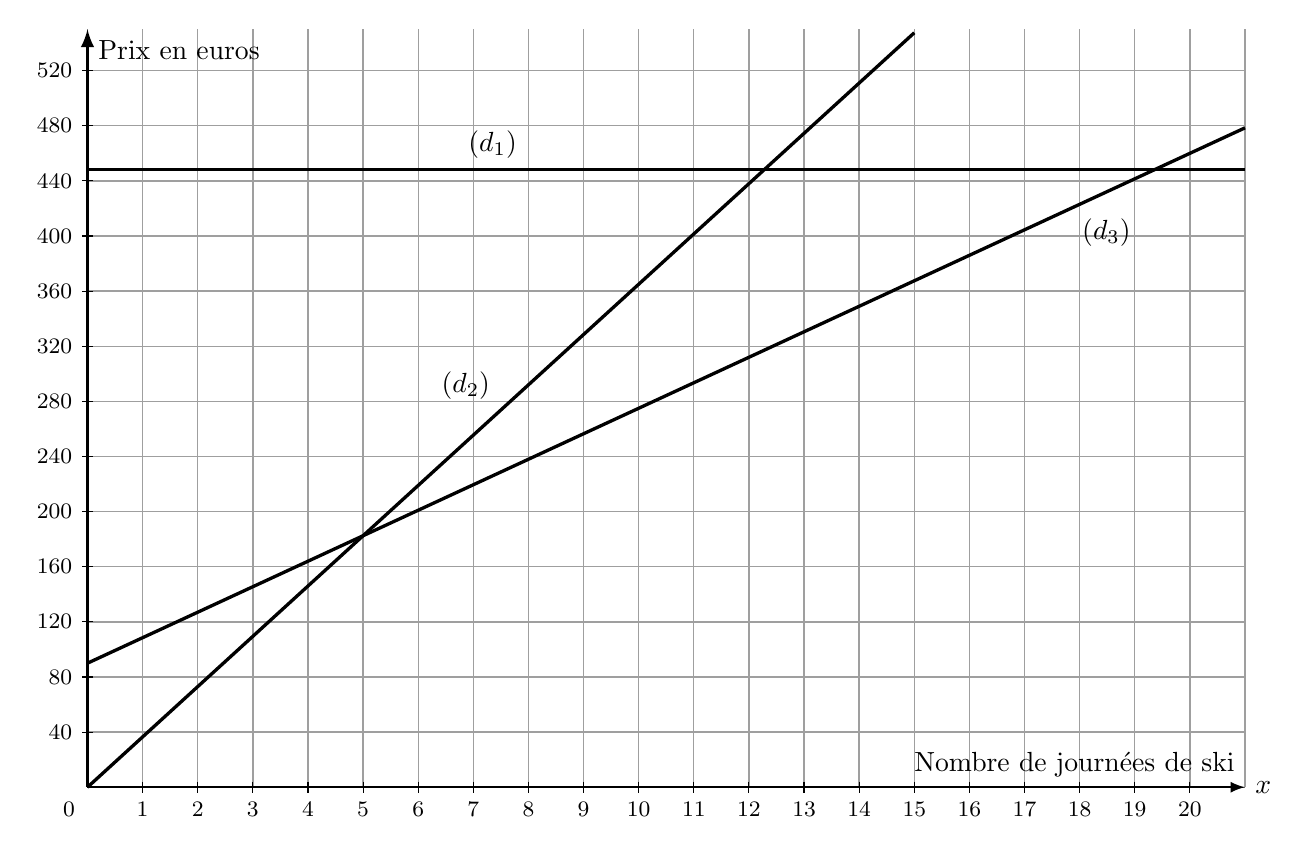
\begin{tikzpicture}[x=7mm,y=0.175mm,>=latex]
	\draw [color = gray!75, line width = 0.5pt, xstep=1, ystep = 40] (0,0) grid (21,550);
	\foreach \x in {1,...,20}
	\draw[shift={(\x,0)},color=black] (0pt,2pt) -- (0pt,-2pt) node[below, fill = white] {\footnotesize $\np{\x}$};
	\foreach \y in {40,80,...,520}
	\draw[shift={(0,\y)},color=black] (2pt,0pt) -- (-2pt,0pt) node[left, fill = white] {\footnotesize $\np{\y}$};
	\draw [->, line width = 0.8pt] (0,0)--(21,0) node[right] {$x$} node[above left] {Nombre de journées de ski};
	
	\draw [->, line width = 1.2pt] (0,0)--(0,550) node[below right] {Prix en euros};
	\draw[color=black] (0-1pt,-2pt) node[below left] {{\footnotesize 0}};
	\draw[line width= 1.2pt] (0,448.50)--(21,448.5) node[pos=.35, above] {$ (d_1) $};
	\draw[line width= 1.2pt] (0,0)--(15,547.5) node[pos=.5, above left] {$ (d_2) $};
	\draw[line width= 1.2pt] (0,90)--(21,478.5) node[pos=.85, below right] {$ (d_3) $};
	
	\end{tikzpicture}

\textbf{Annexe à rendre avec la copie - question 1.}

\begin{center}
	\begin{tabularx}{0.6\linewidth}{|>{\centering \arraybackslash}p{3cm}|*{3}{>{\centering \arraybackslash \rule[-3mm]{0mm}{10mm}}X|}}  \hline
		Nombre de journées de ski&2&6&10\\ \hline
		Formule A & 73 \euro{}&&\\ \hline
		Formule B & 127 \euro{}&&\\ \hline
		Formule C & 448,50 \euro{}&&\\ \hline
		\end{tabularx}
\end{center}
